\documentclass{article}
\usepackage{graphicx}
\usepackage{polski}
\usepackage{enumerate}
\usepackage{titlesec}

\title{Lista 3}
\author{Maciej Kmieciak, 277516}
\date{01.2025}

\begin{document}

\maketitle

\section{Wstęp}

Zaimplementowałem trzy algorytmy:
\begin{itemize}
    \item przecinania pręta w wersjach: naiwnej, ze spamiętywaniem oraz iteracyjnej;
    \item największego wspólnego podciągu w wersjach rekurencyjnej oraz iteracyjnej;
    \item wyboru aktywności w wersjach: rekurencyjnej, iteracyjnej oraz iteracyjnej z użyciem programowania dynamicznego.
\end{itemize}
Poniżej znajdują się kluczowe fragmenty kodów, porównanie działania algorytmów i wnioski. \\ \\
Uwaga: Dla algorytmu wyboru aktywności pierwsze dwa warianty są posortowane wg czasu zakończenia, a ostatni, który używa programowania dynamicznego, wg czasu rozpoczęcia.

\section{Najciekawsze fragmenty kodu}

\subsection{Cut Rod - wersja naiwna}

\begin{verbatim}
int cutRod(int p[], int n) {
    if (n == 0) {
        return 0;
    }

    int q = minInt;
    for (int i = 0; i < n; ++i) {
        q = max(q, p[i] + cutRod(p, n - i - 1));
    }

    return q;
}
\end{verbatim}

W pętli \texttt{for} próbujemy wszystkie możliwe pierwsze cięcia (pierwsze z perpektywy wywołania w którym jesteśmy). Dla każdego z nich, rekurencyjnie liczymy maksymalny zarobek, jaki może nam dać to cięcie i wszystkie kolejne. Zwracamy największą z tych wartości.

\subsection{Cut Rod - wersja ze spamiętywaniem}

\begin{verbatim}
int memorizedCutRod(int p[], int r[], int n) {
    if (r[n] >= 0) {
        return r[n];
    }

    int q = minInt;
    if (n == 0) {
        q = 0;
    }
    else {
        for (int i = 0; i < n; ++i) {
            q = max(q, p[i] + memorizedCutRod(p, r, n - i - 1));
        }
    }

    r[n] = q;
    return q;
}
\end{verbatim}

Tutaj dodajemy tablicę \texttt{r}, w której przechowujemy maksymalny zarobek dla danej długości pręta. Na początku każdego rekurencyjnego wywołania \texttt{memorizedCutRod} sprawdzamy, czy dany wynik został już obliczony wcześniej. Jeśli tak, zwracamy go. Jeśli nie, liczymy maksimum jak wyżej, dodatkowo zapisując nowy wynik do \texttt{r}.

\subsection{Cut Rod - wersja iteracyjna}

\begin{verbatim}
pair<vector<int>, vector<int>> extBotUpCutRod(int p[], int n) {
    vector<int> r(n + 1, 0);
    vector<int> s(n + 1, 0);

    for (int j = 1; j <= n; ++j) {
        int q = minInt;

        for (int i = 1; i <= j; ++i) {
            if (q < p[i - 1] + r[j - i]) {
                q = p[i - 1] + r[j - i];
                s[j] = i;
            }
        }

        r[j] = q;
    }

    return { r, s };
}
\end{verbatim}

W wersji iteracyjnej rozwiązujemy problem najpierw dla krótszych długości pręta. Dla coraz dłuższych prętów sprawdzamy wszystkie możliwe cięcia, odejmując ich długości odczytujemy dotychczasowy maksymalny zarobek i szukamy największego.

\subsection{LCS - wersja rekurencyjna ze spamiętywaniem}

\begin{verbatim}
int LCS_Recursive_Helper(const vector<int>& X, const vector<int>& Y, 
    int i, int j, vector<vector<int>>& memo, vector<vector<string>>& b) {
    
    if (i == 0 || j == 0) return 0;
    if (memo[i][j] != -1) return memo[i][j];

    if (X[i - 1] == Y[j - 1]) {
        memo[i][j] = LCS_Recursive_Helper(X, Y, i - 1, j - 1, memo, b) + 1;
        b[i][j] = "DIAGONAL";
    }
    else {
        int up = LCS_Recursive_Helper(X, Y, i - 1, j, memo, b);
        int left = LCS_Recursive_Helper(X, Y, i, j - 1, memo, b);

        if (up >= left) {
            memo[i][j] = up;
            b[i][j] = "UP";
        }
        else {
            memo[i][j] = left;
            b[i][j] = "LEFT";
        }
    }

    return memo[i][j];
}
\end{verbatim}

Jeśli którykolwiek z ciągów się skończył, zwracamy zero. Jeśli \texttt{memo[i][j]} już ma wartość, zwracamy ją, żeby uniknąć powtórki liczenia. Dalej, jeśli \texttt{X[i-1]} i \texttt{Y[j-1]} są równe, zapisujemy ruch "na skos" i zwiększamy długość wspólnego podciągu o jeden. W przeciwnym wypadku rekurencyjnie liczymy najdłuższe podciągi dla komórki powyżej \texttt{(i - 1, j)} i na lewo \texttt{(i, j - 1)}. Wybieramy dłuższy z nich i zapisujemy jego długość w \texttt{memo}, a kierunek w \texttt{b}.

\subsection{LCS - iteracyjna}

\begin{verbatim}
void Print_Solution_Iterative(const vector<vector<string>>& b, 
    const vector<int>& X, int i, int j) {
    
    if (i == 0 || j == 0) return;
    if (b[i][j] == "DIAGONAL") {
        Print_Solution_Iterative(b, X, i - 1, j - 1);
        cout << X[i - 1] << " ";
    }
    else if (b[i][j] == "UP") {
        Print_Solution_Iterative(b, X, i - 1, j);
    }
    else {
        Print_Solution_Iterative(b, X, i, j - 1);
    }
}
\end{verbatim}

Ten fragment odpowiada za odzyskanie wynikowego podciągu z wykorzystaniem kierunków zapisanych w macierzy \texttt{b}. Osiągnięcie zera którymkolwiek z indeksów oznacza koniec pracy. W przypadku \texttt{DIAGONAL} wiemy, że element \texttt{X[i-1]} jest częścią wyniku (ostanim elementem). Najpierw rekurencyjnie odzyskujemy wynik dla \texttt{(i - 1, j - 1)}, co odpowiada przesunięciu na skos. Na koniec wypisujemy wartość \texttt{X[i - 1]}. Analogicznie w przypadkach \texttt{UP} i \texttt{LEFT} z tą różnicą, że tam nie wypisujemy ostatniego elementu zgodnie z informacją o kierunku.

\subsection{Activity Selector - wersja rekurencyjna}

\begin{verbatim}
vector<int> RecursiveActivitySelector(const vector<int>& s, 
    const vector<int>& f, int k) {
    
    int n = s.size() - 1;
    int m = k + 1;
    while (m <= n && s[m] < f[k]) {
        m++;
    }
    if (m > n) {
        return {};
    }
    vector<int> result = { m };
    vector<int> next = RecursiveActivitySelector(s, f, m);
    result.insert(result.end(), next.begin(), next.end());
    return result;
}
\end{verbatim}

\texttt{k} jest indeksem ostatniej wybranej aktywności (z wyjątkiem pierwszego wywołania). Zaczynając od \texttt{k + 1}, szukamy aktywności, której czas rozpoczęcia jest większy lub równy czasowi zakończenia poprzedniej. Dodajemy ją do tablicy (wektora) i w taki sam sposób szukamy kolejnej. Wiadomo, że takie podejście zawsze da optymalny wybór.

\subsection{Activity Selector - wersja iteracyjna}

\begin{verbatim}
vector<int> IterativeActivitySelector(const vector<int>& s, 
    const vector<int>& f) {
    
    int n = s.size() - 1;
    vector<int> A = { 1 };
    int k = 1;
    for (int m = 2; m <= n; ++m) {
        if (s[m] >= f[k]) {
            A.push_back(m);
            k = m;
        }
    }
    return A;
}
\end{verbatim}

Wersja iteracyjna działa na tej samej zasadzie, co rekurencyjna. Zamiast stosu wywołań mamy odpowiednią pętlę \texttt{for}.

\subsection{Activity Selector - programowanie dynamiczne}

\begin{verbatim}
vector<int> DPActivitySelector(const vector<int>& s, 
    const vector<int>& f) {
    
    int n = s.size() - 1;
    vector<vector<vector<int>>> dp(n + 1, vector<vector<int>>(n + 1));
    for (int i = n; i >= 0; --i) {
        for (int j = i + 1; j <= n; ++j) {
            int m = i + 1;
            while (m <= j && s[m] < f[i]) {
                m++;
            }
            vector<int> exclude = dp[i + 1][j];
            vector<int> include = (i > 0) ? vector<int>{i} : vector<int>{};
            if (m <= j) {
                include.insert(include.end(), dp[m][j].begin(), dp[m][j].end());
            }
            dp[i][j] = (include.size() > exclude.size()) ? include : exclude;
        }
    }
    vector<int> result = dp[0][n];
    if (!result.empty() && result[0] == 0) {
        result.erase(result.begin());
    }
    return result;
}
\end{verbatim}

\texttt{dp[i][j]} odpowiada optymalnemu wyborowi aktywności pomiędzy indeksami \texttt{i} oraz \texttt{j}. Dla każdej pary \texttt{(i, j)} sprawdzamy, czy zawrzeć aktywność \texttt{i}, czy nie. Jeśli mamy zawrzeć obecną aktywność \texttt{i} (tablica \texttt{include}), dodajemy ją do \texttt{dp[m][j]}, o ile to możliwe, ponieważ kolejna aktywność musi zaczynać się po zakończeniu poprzedniej. Jeśli nie, po prostu bierzemy \texttt{dp[i+1][j]} jako tablicę \texttt{exclude}. Porównujemy rozmiary \texttt{include} i \texttt{exclude}, biorąc większą z dwóch. To znaczy, że rozwiązanie \texttt{dp[i][j]} zależy od podproblemów \texttt{dp[i+1][j]} oraz \texttt{dp[m][j]}. Ostateczne rozwiązanie, po przejściu wszystkich aktywności znajdzie się w \texttt{dp[0][n]}.

\section{Porównanie działania algorytmów}

\subsection{Cut Rod}

\begin{center}
    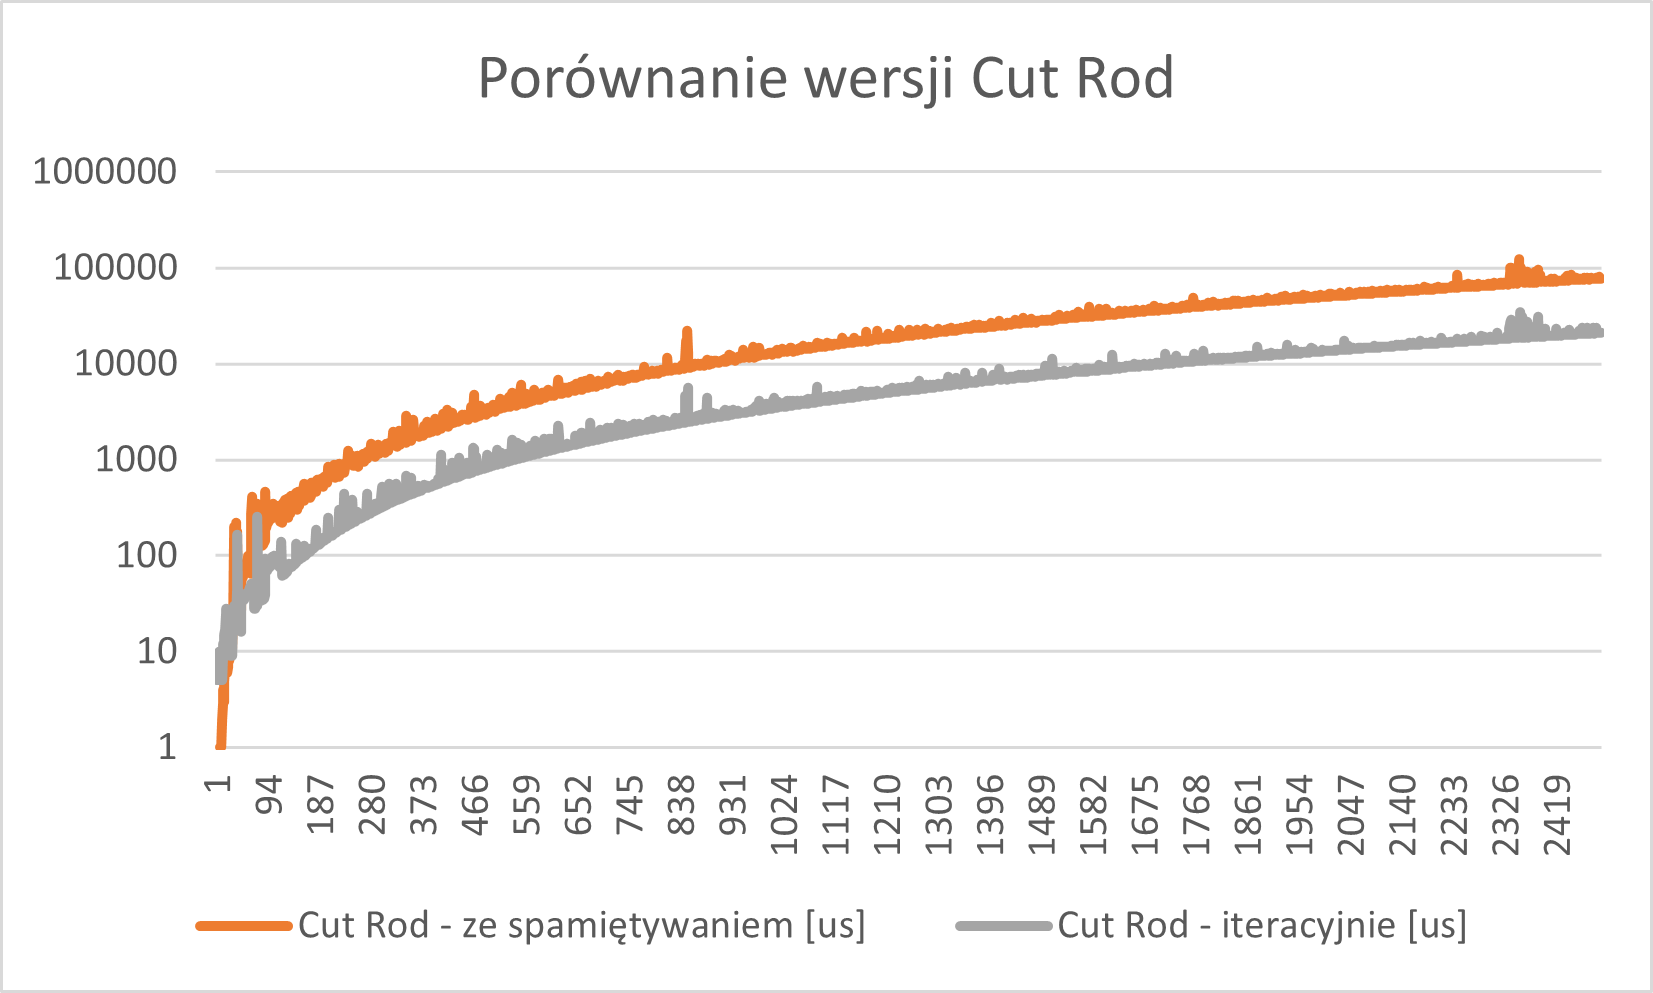
\includegraphics[width=1\textwidth]{Cut Rod.png}
\end{center}

\begin{center}
\begin{tabular}{c|c}
    \hline
    n & Cut Rod - rekurencyjnie ($\mu$s) \\
    \hline
    1 & 0 \\
    2 & 0 \\
    3 & 2 \\
    4 & 1 \\
    5 & 2 \\
    6 & 34 \\
    7 & 4 \\
    8 & 34 \\
    9 & 19 \\
    10 & 38 \\
    11 & 72 \\
    12 & 142 \\
    13 & 295 \\
    14 & 479 \\
    15 & 1081 \\
    16 & 3192 \\
    17 & 5627 \\
    18 & 12501 \\
    19 & 21158 \\
    20 & 37913 \\
    21 & 61524 \\
    22 & 134463 \\
    23 & 318141 \\
    24 & 637419 \\
    25 & 1174241 \\
    \hline
\end{tabular}
\end{center}

Cut Rod w wersji naiwnej jest skrajnie mało wydajny ze względu na ciągłe powtórki. Gdy dodamy spamiętywanie, wydajność znacznie wzrasta. Dalej, wersja rekurencyjna jest wyraźnie wolniejsza niż iteracyjna, ze względu na operacje związane z przetwarzaniem stosu wywołań.

\subsection{LCS}

\begin{center}
    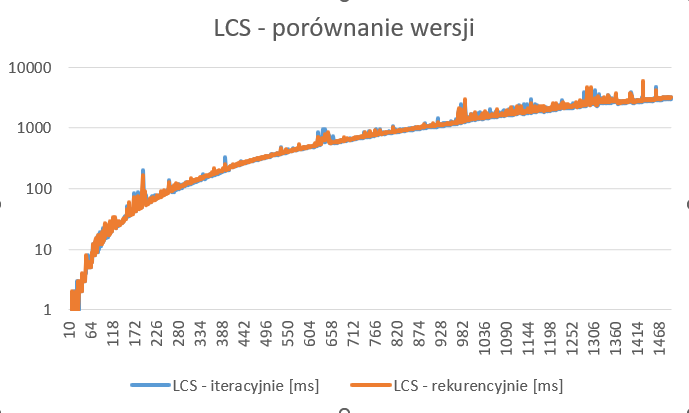
\includegraphics[width=1\textwidth]{LCS.png}
\end{center}

W przypadku LCS wersje iteracyjne i rekurencyjne działają w podobnym czasie, nie widać przewagi podejścia iteracyjnego. Można przypuszczać, że stos wywołań tu jest relatywnie mało istotny dla czasu wykonania.

\subsection{Activity Selector}

\begin{center}
    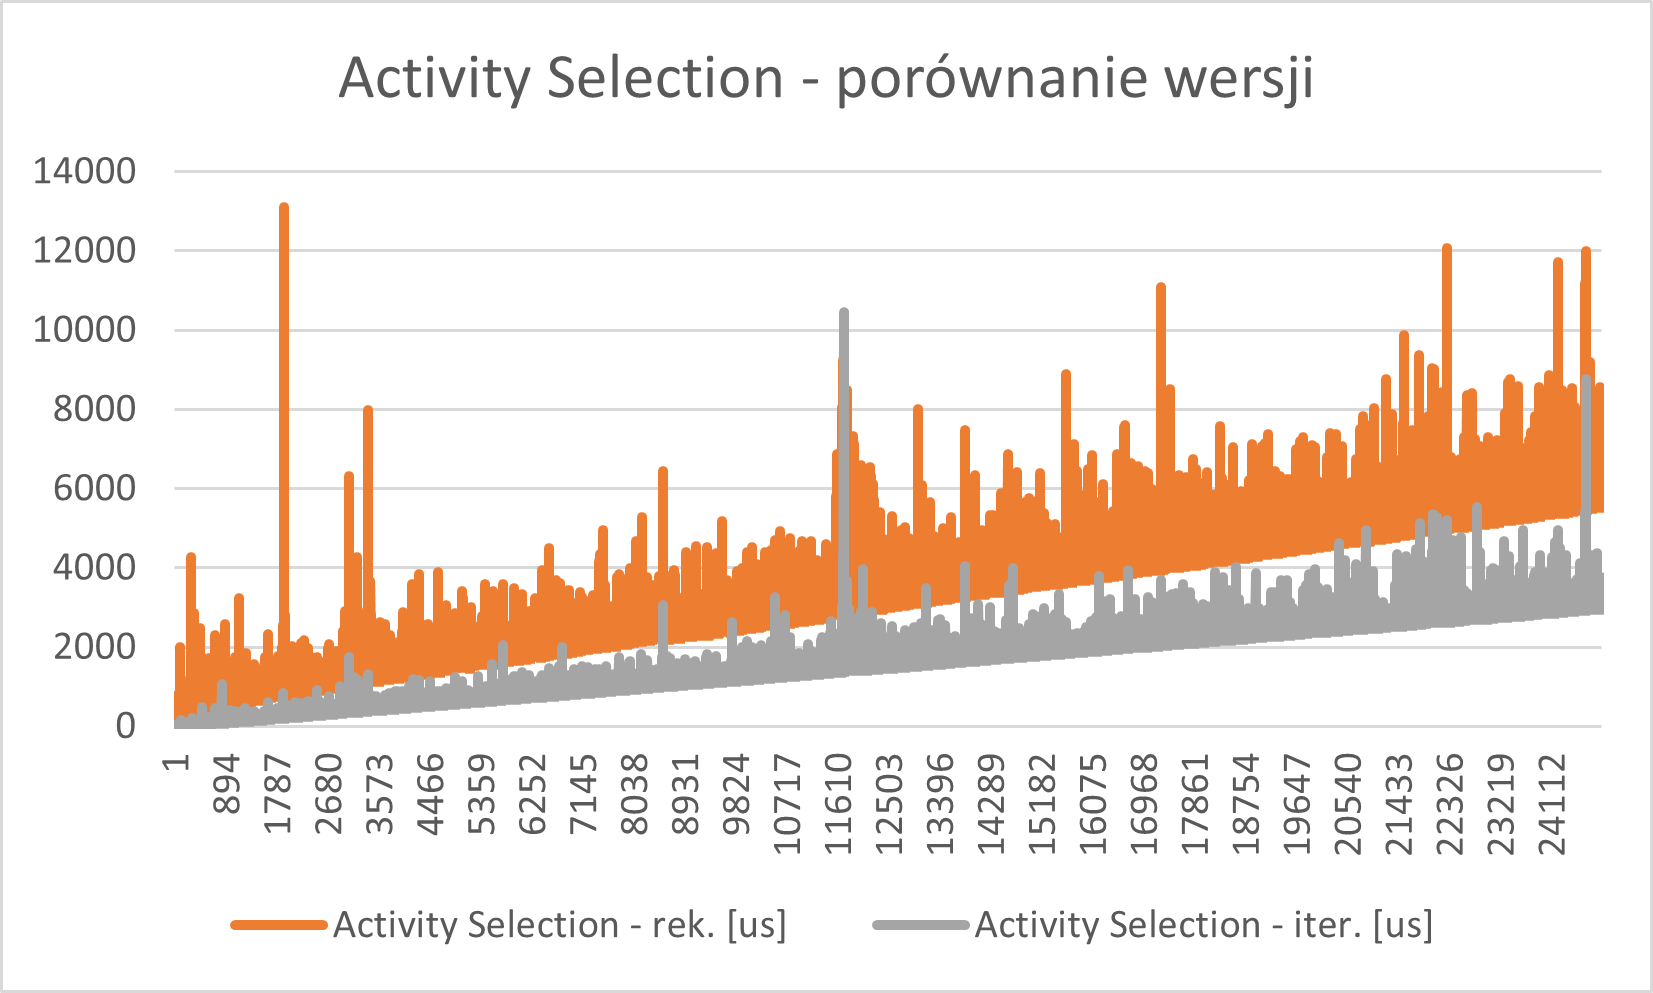
\includegraphics[width=1\textwidth]{Activity Selection.png}

\begin{tabular}{c|c}
     \hline
     n & Activity Selector - prog. dyn. (ms) \\
     \hline
    10         & 0                   \\
    100        & 26                  \\
    200        & 108                 \\
    300        & 259                 \\
    400        & 491                 \\
    500        & 810                 \\
    600        & 1301                \\
    700        & 1795                \\
    800        & 2486                \\
    1000       & 4271                \\
    \hline
\end{tabular}
\end{center}

W przypadku Activity Selector, czas wykonania dla wersji z użyciem programowania dynamicznego rośnie w przybliżeniu kwadratowo, podczas gdy dla dwóch pierwszych wersji rośnie liniowo. Dodatkowo, ponownie, wersja iteracyjna jest szybsza niż rekurencyjna.

\section{Wnioski}

Na podstawie powyższych danych wydaje się, że rekurencyjne wersje wielu algorytmów działają gorzej (a przynajmniej nie lepiej) niż iteracyjne, ze względu na konieczność utworzenia stosu wywołań i przejścia przez niego. Zużywają też więcej pamięci, a dla dużych danych stwarzają ryzyko zajęcia całej dostępnej pamięci lub wygenerowania błędu przepełnienia stosu. Oczywiście, widać też, że kluczowe jest unikanie powtórek obliczeń (naiwny Cut Rod) oraz dostosowanie podejścia do charakterystyki problemu (Activity Selector i programowanie dynamiczne).

\end{document}
